\documentclass[11pt]{article}
\usepackage[left=1in,right=1in,top=1in,bottom=1in]{geometry}
\usepackage{amsmath,amssymb}
\usepackage{booktabs}
\usepackage[round]{natbib}
\usepackage{hyperref}
\hypersetup{colorlinks,citecolor=blue,filecolor=blue,linkcolor=blue,urlcolor=blue}
\usepackage{graphicx}
\usepackage{float}
\usepackage[ruled,lined]{algorithm2e}
\usepackage{xcolor}
\usepackage{subcaption}
\usepackage{url}
\usepackage{microtype}

% Custom commands
\DeclareMathOperator*{\argmin}{arg\,min}
\DeclareMathOperator*{\argmax}{arg\,max}
\newcommand{\E}{\mathbb{E}}
\newcommand{\R}{\mathbb{R}}

\title{EconIRL: Estimators for Understanding and Predicting\\ Dynamic Discrete Choices}

\author{
  Pranjal Rawat\thanks{PhD Candidate, Georgetown University. \href{mailto:pp712@georgetown.edu}{pp712@georgetown.edu}}
  \and
  John Rust\thanks{Professor, Georgetown University. \href{mailto:jf693@georgetown.edu}{jf693@georgetown.edu}}
}

\date{\today}

\begin{document}

\maketitle

\begin{abstract}
\noindent
EconIRL implements twelve estimators for dynamic discrete choice models spanning structural econometrics (NFXP, CCP, MPEC) and inverse reinforcement learning (MCE-IRL, AIRL, GLADIUS).
All estimators share a common interface and feed into unified post-estimation infrastructure for standard errors, identification diagnostics, and counterfactual simulation.
We show that the IQ-Learn chi-squared objective is algebraically equivalent to a penalized conditional log-likelihood in the tabular DDC setting, connecting occupancy-matching IRL to structural maximum likelihood estimation.
Three simulation studies validate the package: a tabular benchmark where all structural and IRL estimators converge to the same solution, a high-dimensional state space where sieve and neural methods maintain accuracy at lower computational cost, and a nonlinear reward environment where deep IRL outperforms linear models.
The library is built on JAX for automatic differentiation and GPU acceleration and is MIT-licensed.
\end{abstract}

\bigskip

\section{Introduction}

Dynamic discrete choice models in economics and inverse reinforcement learning in computer science solve the same fundamental inference problem. An agent makes a sequence of decisions over time, and the researcher observes these decisions and wants to recover the reward function that rationalizes them. \citet{rust1987} formalized this problem as nested fixed-point maximum likelihood estimation, and the structural econometrics literature that followed developed a rich family of estimators including conditional choice probability methods and mathematical programming approaches \citep{aguirregabiriaMira2010}. Independently, \citet{ziebart2010} formalized the same problem as maximum causal entropy inverse reinforcement learning, and the machine learning literature developed its own family of estimators including adversarial methods and soft Q-learning. These two traditions share the same Bellman equation, the same discount factor, and the same logit choice kernel, yet they developed with different notation, different software ecosystems, and no unified pipeline for statistical inference or counterfactual analysis.

Existing software does not bridge these traditions. The \texttt{imitation} library \citep{gleave2022} implements several IRL algorithms but provides no standard errors, no identification diagnostics, and no counterfactual simulation. Stata packages for dynamic discrete choice cover NFXP and a handful of related estimators but cannot accommodate neural reward functions or adversarial training. There is no library where a practitioner can specify a DDC model once, swap between structural and IRL estimators, and obtain valid inference from all of them through a single API. This gap forces applied researchers to maintain separate codebases for each estimator, making systematic comparison across methods unnecessarily difficult.

This paper introduces EconIRL, a Python library that provides twelve estimators for dynamic discrete choice models through a common \texttt{Estimator} protocol. Six estimators come from structural econometrics (NFXP, CCP, MPEC, NNES, SEES, TD-CCP) and six from inverse reinforcement learning (MCE-IRL, Deep MaxEnt, AIRL, GLADIUS, IQ-Learn, Behavioral Cloning). Every estimator returns an \texttt{EstimationSummary} object that provides standard errors by four methods (analytical, bootstrap, jackknife, and sandwich), identification diagnostics, and counterfactual simulation. The library is built on JAX \citep{jax2018} for automatic differentiation through fixed-point solvers via implicit differentiation, with Equinox \citep{kidger2021} for neural network components. We also present a new theoretical result connecting the IQ-Learn chi-squared divergence objective to a penalized conditional log-likelihood in the tabular DDC setting \citep{rawat2026}, which provides a formal bridge between occupancy-matching IRL and structural maximum likelihood estimation. Three simulation studies validate convergence, scaling, and nonlinear reward recovery across estimator families. The library is MIT licensed and pip-installable.

The remainder of the paper is organized as follows. Section~\ref{sec:framework} sets up notation and describes the dynamic discrete choice model that serves as the common foundation for all estimators. Section~\ref{sec:estimators} describes each estimator with pseudocode and references to the underlying theory. Section~\ref{sec:iq_learn} presents the IQ-Learn equivalence result. Section~\ref{sec:post_estimation} covers the post-estimation infrastructure for inference, diagnostics, and counterfactual analysis. Section~\ref{sec:experiments} presents three simulation case studies and real-data applications. Section~\ref{sec:conclusion} concludes.

\section{Framework}
\label{sec:framework}

\paragraph{The DDC model.}
An agent observes a discrete state $s_t \in \mathcal{S}$ at each period $t$, chooses an action $a_t \in \mathcal{A}$, and receives a flow payoff $u(s_t, a_t; \theta) + \sigma\,\epsilon_{t,a}$, where $\epsilon_{t,a}$ follows a Type~I extreme value distribution. The state evolves according to a known transition kernel $P(s' \mid s, a)$, and the agent discounts future payoffs at rate $\beta \in [0,1)$. This is the dynamic discrete choice framework introduced by \citet{rust1987}. The agent's choice-specific value function satisfies the Bellman equation
\begin{equation}
\label{eq:bellman}
Q(s,a;\theta) \;=\; u(s,a;\theta) \;+\; \beta \sum_{s' \in \mathcal{S}} P(s' \mid s,a)\, V(s'),
\end{equation}
where the integrated value function takes the log-sum-exp form implied by the extreme value error
\begin{equation}
\label{eq:smoothed_max}
V(s) \;=\; \sigma \log \sum_{a \in \mathcal{A}} \exp\!\bigl(Q(s,a;\theta)/\sigma\bigr).
\end{equation}
The optimal policy is the softmax over choice-specific values
\begin{equation}
\label{eq:softmax_policy}
\pi(a \mid s;\theta) \;=\; \frac{\exp\!\bigl(Q(s,a;\theta)/\sigma\bigr)}{\sum_{a' \in \mathcal{A}} \exp\!\bigl(Q(s,a';\theta)/\sigma\bigr)}.
\end{equation}
This system is simultaneously the structural logit model of econometrics and the maximum causal entropy policy of \citet{ziebart2010}. The structural side views Equations~\eqref{eq:bellman}--\eqref{eq:softmax_policy} as a likelihood model and estimates $\theta$ by maximum likelihood. The IRL side views them as a forward model mapping reward weights to behavior and estimates $\theta$ by matching observed and predicted feature expectations. The mathematical content is the same.

\paragraph{Identification.}
Rewards in this model are identified only up to additive state-dependent constants and global scale. For any bounded function $h \colon \mathcal{S} \to \mathbb{R}$, the shaped reward
\begin{equation}
\label{eq:reward_shaping}
r'(s,a) \;=\; r(s,a) \;+\; h(s) \;-\; \beta \sum_{s' \in \mathcal{S}} P(s' \mid s,a)\, h(s')
\end{equation}
yields the same optimal policy as the original reward $r(s,a)$ \citep{ng1999, magnacThesmar2002, kim2021}. This invariance means that raw reward magnitudes are not recoverable without further restrictions. The package resolves this ambiguity in three ways depending on the estimator family.

\begin{table}[H]
\centering
\small
\caption{Identification strategies across estimator families.}
\label{tab:identification}
\begin{tabular}{lll}
\toprule
Strategy & Estimators & What is Recovered \\
\midrule
Parametric $u = \theta^\top \phi(s,a)$ & NFXP, CCP, MPEC, NNES, TD-CCP, SEES & $\theta$ (structural parameters) \\
Feature matching + norm & MCE-IRL & $\theta$ (reward weights) \\
Disentanglement & AIRL & $r(s)$ (state-only reward) \\
\bottomrule
\end{tabular}
\end{table}

First, structural estimators restrict the flow utility to a linear-in-parameters form $u(s,a;\theta) = \theta^\top \phi(s,a)$, where $\phi$ is a known feature map. The parametric structure pins down the reward up to $\theta$, and the likelihood identifies $\theta$ under standard rank conditions on the feature matrix. Second, MCE-IRL estimates reward weights $\theta$ by matching empirical and model-implied feature expectations, with a norm constraint or regularization penalty that resolves the scale ambiguity. Third, AIRL separates the discriminator into a state-only reward and a shaping potential, recovering $r(s)$ up to a constant by construction \citep{fu2018}. Table~\ref{tab:identification} summarizes these three strategies.

\paragraph{Software abstractions.}
The library encodes the primitives above through three core types. \texttt{DDCProblem} is a frozen dataclass that stores the number of states $|\mathcal{S}|$, the number of actions $|\mathcal{A}|$, the discount factor $\beta$, and the scale parameter $\sigma$. Every estimator receives this object and uses it to construct value iteration operators and policy mappings. \texttt{Panel} is a list of \texttt{Trajectory} objects, where each trajectory records a sequence of state-action pairs $(s_t, a_t)$ observed from a single agent. The panel structure preserves the serial dependence within trajectories while allowing estimators to treat agents as independent. The \texttt{Estimator} protocol requires every estimator to implement a single method, \texttt{.estimate(panel, utility, problem, transitions)}, and return an \texttt{EstimationSummary}. This API contract means that all twelve estimators are interchangeable parts. A user can swap NFXP for MCE-IRL or AIRL for CCP with one line of code and receive standard errors, identification diagnostics, and counterfactual predictions through the same post-estimation pipeline regardless of which estimator produced them.

\section{Estimators}
\label{sec:estimators}

EconIRL implements twelve estimators organized into three families.
The classical structural estimators (NFXP, CCP, MPEC) solve the forward problem exactly on tabular state spaces.
The neural structural estimators (NNES, TD-CCP, SEES) approximate the value function to scale beyond tabular.
The inverse reinforcement learning estimators (MCE-IRL, AIRL, GLADIUS, f-IRL, IQ-Learn) recover rewards from demonstrations, with behavioral cloning as a non-structural baseline.
Table~\ref{tab:estimators} summarizes the capability of each method.

\begin{table}[t]
\centering
\caption{Estimator summary. ``Direction'' indicates whether the estimator solves the forward problem (parameters to policy) or the inverse problem (demonstrations to reward). ``Needs $P$'' indicates whether known transition matrices are required. ``SEs'' indicates whether valid standard errors are available.}
\label{tab:estimators}
\small
\begin{tabular}{lllcccc}
\toprule
Estimator & Reference & Direction & Needs $P$ & SEs & Scales & Transfer \\
\midrule
NFXP-NK    & \citet{rust1987, iskhakov2016}        & Forward & Yes & Analytical & No  & No \\
CCP-NPL    & \citet{hotzMiller1993, aguirregabiriaMira2002} & Forward & Yes & Hessian    & No  & No \\
MPEC       & \citet{suJudd2012}                     & Forward & Yes & Hessian    & No  & No \\
\midrule
NNES       & \citet{nguyen2025}                     & Forward & Yes & Valid      & Yes & No \\
TD-CCP     & \citet{adusumilliEckardt2025}          & Forward & No  & Robust     & Yes & No \\
SEES       & \citet{luoSang2024}                    & Forward & Yes & Marginal   & Yes & No \\
\midrule
MCE-IRL    & \citet{ziebart2010}                    & Inverse & Yes & Bootstrap  & No  & No \\
AIRL       & \citet{fu2018}                         & Inverse & No  & No         & No  & Yes \\
GLADIUS    & \citet{kang2025}                       & Inverse & Yes & Projected  & Yes & No \\
f-IRL      & \citet{ni2022}                         & Inverse & Yes & No         & No  & No \\
IQ-Learn   & \citet{garg2021}                       & Inverse & Yes & No         & No  & No \\
BC         & \citet{pomerleau1991}                  & Imitation & No & No        & No  & No \\
\bottomrule
\end{tabular}
\end{table}


\subsection{Classical Structural Estimators}

\paragraph{NFXP-NK.}
The nested fixed point algorithm maximizes the exact log-likelihood $\ell(\theta) = \sum_i \log \pi(a_i | s_i; \theta)$ where choice probabilities come from solving the Bellman equation to machine precision at each outer step.
The inner loop uses the SA-then-NK polyalgorithm of \citet{iskhakov2016}, which starts with successive approximation for global convergence and switches to Newton-Kantorovich near the fixed point for quadratic convergence.
Gradients of the log-likelihood with respect to $\theta$ are computed analytically via the implicit function theorem, differentiating through the Bellman fixed point without backpropagation or finite differences.
The outer loop uses BHHH optimization, which guarantees a positive-definite Hessian approximation from the outer product of per-observation score vectors.
Algorithm~\ref{alg:nfxp} shows the main loop.

\begin{algorithm}[t]
\DontPrintSemicolon
\caption{NFXP-NK \citep{rust1987, iskhakov2016}}
\label{alg:nfxp}
\KwIn{Panel $\mathcal{D}$, features $\phi$, transitions $P$, discount $\beta$}
Initialize $\theta_0$\;
\For{$k = 0, 1, 2, \ldots$}{
  \textbf{Inner loop:} Solve $V = T(V; \theta_k)$ via SA then NK\;
  Compute $Q(s,a) = u(s,a;\theta_k) + \beta \sum_{s'} P(s'|s,a)\, V(s')$\;
  Compute $\pi(a|s) = \mathrm{softmax}(Q/\sigma)$\;
  Compute $\nabla_\theta \ell$ via implicit differentiation\;
  Update $\theta_{k+1}$ via BHHH or L-BFGS-B\;
  \lIf{$\|\nabla \ell\| < \varepsilon$}{\textbf{break}}
}
\KwOut{$\hat\theta$, $V^*$, $\pi^*$, $(-H)^{-1}$ for analytical SEs}
\end{algorithm}

\paragraph{CCP-NPL.}
The Hotz-Miller inversion lemma \citep{hotzMiller1993} shows that under additive separability and IID extreme value shocks, observed choice probabilities $\hat P(a|s)$ uniquely invert to value differences via the emax correction $e(s,a) = \gamma_{\text{Euler}} - \log \hat P(a|s)$.
This eliminates the inner Bellman loop entirely.
Value recovery reduces to a single matrix inversion $(I - \beta F_\pi)^{-1}$, which costs $O(|\mathcal{S}|^3)$ once compared to thousands of value iterations in NFXP.
\citet{aguirregabiriaMira2002} show that iterating the Hotz-Miller inversion in CCP space (nested pseudo-likelihood, or NPL) converges to the MLE when the equilibrium is Lyapunov stable.
Setting $K=1$ gives a consistent but inefficient estimator.
Setting $K=5$ to $10$ recovers full MLE efficiency.
CCP-NPL is the only method in this package that extends naturally to dynamic games where computing Nash equilibria is infeasible.

\paragraph{MPEC.}
The mathematical programming with equilibrium constraints approach of \citet{suJudd2012} treats the value function $V(s)$ as explicit decision variables alongside the structural parameters $\theta$.
The Bellman equation $V = T(V;\theta)$ becomes a set of equality constraints enforced via an augmented Lagrangian.
This eliminates the inner loop entirely and jointly optimizes $(\theta, V)$ in a single L-BFGS-B call with increasing penalty on constraint violation.
On the Rust bus benchmark at $\beta = 0.95$, MPEC achieves identical parameter estimates to NFXP while running six to nine times faster.


\subsection{Neural Structural Estimators}

\paragraph{NNES.}
The neural network estimation of structural models approach of \citet{nguyen2025} uses a two-phase procedure.
In Phase 1 a neural network $V_\phi$ is trained to approximate the NPL Bellman target using data CCPs and the Hotz-Miller emax correction.
In Phase 2 the learned $V_\phi$ is plugged into the CCP log-likelihood and the structural parameters $\theta$ are optimized via L-BFGS-B.
The key theoretical contribution is the zero Jacobian property (Proposition 1): at the true CCP, $\partial \phi_{\theta_0}(P^*, V^*)/\partial P = 0$, so neural network errors in $V$ have only second-order effects on the likelihood.
This Neyman orthogonality guarantees that $\hat\theta$ is $\sqrt{n}$-consistent even when $V_\phi$ converges at the slower rate $o_p(n^{-1/4})$, and the estimator achieves the semiparametric efficiency bound without bias correction or cross-fitting.

\paragraph{TD-CCP.}
The temporal-difference CCP estimator of \citet{adusumilliEckardt2025} is the only method in this package that does not require known or estimated transition densities.
The key insight is that the CCP value function components $h(a,x)$ and $g(a,x)$ can be characterized via temporal-difference fixed-point equations that depend only on sample expectations over observed transitions $(s, a, s')$, not on the density $p(s'|s,a)$.
Algorithm~\ref{alg:tdccp} shows the linear semi-gradient variant, which solves for $h$ via a single matrix inversion.

\begin{algorithm}[t]
\DontPrintSemicolon
\caption{TD-CCP, linear semi-gradient \citep{adusumilliEckardt2025}}
\label{alg:tdccp}
\KwIn{Panel $\mathcal{D}$ with transitions $(s_t, a_t, s_{t+1})$, features $\phi$, basis $\Psi$}
Estimate CCPs $\hat P(a|s)$ from data frequencies\;
\For{each action $a$ and feature $k$}{
  Solve $(I - \beta \hat F_\pi)\, h_{a,k} = \phi_{a,k}$ via matrix inversion\;
}
Construct pseudo-outcome $Y_i = \sum_k \theta_k\, h_k(a_i, x_i)$\;
Minimize pseudo-likelihood over $\theta$ via GMM\;
Compute robust SEs via locally debiased moment condition\;
\KwOut{$\hat\theta$, robust SEs valid at $\sqrt{n}$-rate}
\end{algorithm}

The locally robust moment condition (Theorem 5 of \citealt{adusumilliEckardt2025}) uses a backward value function $\lambda$ and debiased moment $\zeta$ to correct for first-stage estimation error, producing standard errors valid at parametric rates despite nonparametric first stages.
The per-feature $h(a,x)$ decomposition also provides interpretable diagnostics showing how each feature contributes to the value function.

\paragraph{SEES.}
The sieve estimator of \citet{luoSang2024} approximates $V(s) \approx \Psi(s)\,\alpha$ where $\Psi$ is a deterministic sieve basis of Fourier or polynomial functions.
Joint L-BFGS-B optimization over $(\theta, \alpha)$ with an $\ell^2$ penalty on $\alpha$ enforces Bellman consistency without ever solving a fixed point.
The basis matrix is deterministic and continuation values reduce to a single matrix multiply $P_a \Psi$, making the computational cost $O(\text{basis\_dim})$ independent of $|\mathcal{S}|$.
On the Rust bus benchmark, SEES achieves parameter estimates within one percent of NFXP while running fifteen to thirty-four times faster.
No neural network training is involved.


\subsection{Inverse Reinforcement Learning Estimators}

\paragraph{MCE-IRL.}
Maximum causal entropy IRL \citep{ziebart2010} is the bridge estimator connecting the econometrics and machine learning traditions.
The backward pass runs soft value iteration to compute $V$, $Q$, and $\pi$ from the current reward weights $\theta$.
The forward pass computes state visitation frequencies $D_\pi$ via the occupancy measure fixed point $(I - \beta P_\pi^\top)^{-1}\rho_0$.
The gradient is the feature matching residual $\nabla_\theta \mathcal{L} = \E_{\text{data}}[\phi] - \E_\pi[\phi]$.
Algorithm~\ref{alg:mceirl} shows the main loop.

\begin{algorithm}[t]
\DontPrintSemicolon
\caption{MCE-IRL \citep{ziebart2010}}
\label{alg:mceirl}
\KwIn{Panel $\mathcal{D}$, features $\phi$, transitions $P$, discount $\beta$}
Compute empirical features $\bar f = \frac{1}{N}\sum_i \phi(s_i, a_i)$\;
Initialize $\theta_0$\;
\For{$k = 0, 1, 2, \ldots$}{
  \textbf{Backward:} Soft VI $\to$ $V$, $Q$, $\pi$ from $\theta_k$\;
  \textbf{Forward:} $D_\pi = (I - \beta P_\pi^\top)^{-1}\,\rho_0$\;
  $\bar f_\pi = \sum_s D_\pi(s) \sum_a \pi(a|s)\,\phi(s,a)$\;
  $g = \bar f - \bar f_\pi$ \tcp*{feature matching residual}
  $\theta_{k+1} = \theta_k + \alpha\, g$\;
  \lIf{$\|g\| < \varepsilon$ \textbf{and} $\|D_\pi - D_{\text{data}}\|_\infty < \tau$}{\textbf{break}}
}
\KwOut{$\hat\theta$ (reward weights), bootstrap SEs}
\end{algorithm}

This gradient is simultaneously the MCE gradient of \citet{ziebart2010} and the score of the DDC conditional logit likelihood.
An economist sees structural logit with feature matching.
A machine learning researcher sees maximum entropy IRL.
They solve the same optimization problem.
The deep variant replaces $\theta^\top\phi(s,a)$ with a neural network $r_\psi(s,a)$ following \citet{wulfmeier2016}, gaining flexibility at the cost of interpretability and standard errors.

\paragraph{AIRL.}
Adversarial inverse reinforcement learning \citep{fu2018} is the only IRL method in this package with a proven transfer guarantee.
The discriminator takes the form $D(s,a,s') = \exp(f)/(\exp(f) + \pi(a|s))$ where $f(s,a,s') = g_\psi(s) + \beta\, h_\psi(s') - h_\psi(s)$.
This structure disentangles the state-only reward $g(s)$ from the shaping potential $h(s)$.
Algorithm~\ref{alg:airl} shows the adversarial training loop.

\begin{algorithm}[t]
\DontPrintSemicolon
\caption{AIRL \citep{fu2018}}
\label{alg:airl}
\KwIn{Expert demonstrations $\mathcal{D}_E$, transitions $P$, discount $\beta$}
Initialize reward $g_\psi$, shaping $h_\psi$, policy $\pi_\omega$\;
\For{$k = 0, 1, 2, \ldots$}{
  $f(s,a,s') = g_\psi(s) + \beta\, h_\psi(s') - h_\psi(s)$\;
  $D(s,a,s') = \exp(f) \,/\, \bigl(\exp(f) + \pi_\omega(a|s)\bigr)$\;
  Update $\psi$: $\max_\psi\; \E_{\mathcal{D}_E}[\log D] + \E_\pi[\log(1-D)]$\;
  Update $\omega$: policy improvement against $f$\;
  \lIf{converged}{\textbf{break}}
}
\KwOut{$g_\psi(s)$ (disentangled reward, transfers across environments)}
\end{algorithm}

Theorem 5.1 of \citet{fu2018} proves that the state-only reward recovered by AIRL is disentangled with respect to all dynamics, meaning it transfers across environments with different transition functions.
This is the method to use when rewards learned in simulation must be deployed under different real-world dynamics.

\paragraph{GLADIUS.}
The ERM-IRL estimator of \citet{kang2025} parameterizes $Q(s,a)$ and $\zeta(s,a) = \E[V(s')|s,a]$ with neural networks and trains them with alternating mini-batch SGD.
Even-numbered batches update $\zeta$ via MSE against $\log\sum\exp(Q)$.
Odd-numbered batches update $Q$ via the negative log-likelihood.
After convergence, structural parameters are recovered via action-difference projection $\hat\theta = (\Delta\Phi^\top\Delta\Phi)^{-1}\Delta\Phi^\top\Delta Q$ where $\Delta$ denotes differences from a reference action, eliminating the unidentified additive constant.
A known limitation is that $Q$ is identified only up to a state-dependent constant $c(s)$ that leaks through asymmetric transitions, producing systematic bias in the operating cost parameter on the Rust bus benchmark.

\paragraph{f-IRL.}
The f-IRL estimator of \citet{ni2022} minimizes the $f$-divergence $D_f(\rho_E \| \rho_\pi)$ between expert and policy state-action occupancy measures over a tabular reward function.
The choice of $f$ provides a menu of robustness properties.
KL divergence gives maximum likelihood equivalence.
Chi-squared divergence gives variance sensitivity.
Total variation gives robustness to outlier demonstrations.
No features need to be specified.

\paragraph{IQ-Learn.}
The IQ-Learn estimator of \citet{garg2021} collapses the min-max IRL problem to a concave maximization over $Q$ alone, since the optimal policy is deterministically the softmax of $Q$.
Reward is recovered via the inverse Bellman operator $r(s,a) = Q(s,a) - \beta\sum_{s'} V(s')\,p(s'|s,a)$.
Section~\ref{sec:iq_learn} shows that in the tabular DDC setting this objective is algebraically equivalent to a penalized conditional log-likelihood.

\paragraph{BC (baseline).}
Behavioral cloning \citep{pomerleau1991} estimates the policy directly via frequency counting $\hat P(a|s) = N(s,a)/N(s)$.
No transitions, no Bellman equation, no reward function, and no value function are involved.
\citet{ross2011} show that BC error compounds quadratically under distribution shift at rate $O(T^2\varepsilon)$.
Any IRL method that cannot outperform BC has not learned from MDP structure.
BC establishes the floor for every benchmark in this paper.

\section{Post-Estimation Infrastructure}
\label{sec:post_estimation}

EconIRL provides four methods for computing standard errors on estimated parameters. Asymptotic standard errors use the inverse of the negative Hessian, $\mathrm{Var}(\hat\theta) = (-H)^{-1}$, which is valid under correct specification of the likelihood. Robust sandwich standard errors account for potential misspecification by computing $H^{-1} B H^{-1}$, where $B$ is the outer product of per-observation score vectors. Nonparametric bootstrap standard errors resample trajectories with replacement and re-estimate the model on each bootstrap sample, yielding confidence intervals that do not rely on asymptotic normality. Clustered standard errors aggregate the score vectors within individuals before forming the outer product, accounting for within-individual serial correlation in panel data. The Hessian is computed analytically for NFXP via implicit differentiation through the Bellman fixed point following \citet{iskhakov2016}, and numerically via central finite differences for all other estimators.

The library runs four identification diagnostics before estimation begins. Feature matrix rank is computed on the flattened feature matrix of dimension $(|\mathcal{S}| \times |\mathcal{A}|) \times K$, and if the rank falls below the number of parameters $K$, the model is under-identified and estimation is halted. The condition number of the feature matrix flags near-collinearity that inflates standard errors even when the matrix is technically full rank, with values above $10^6$ triggering a warning. State coverage reports how many of the $|\mathcal{S}|$ states have at least one observation in the data, because states with zero observations produce degenerate CCP estimates that cannot inform the likelihood. Single-action state counts identify states where only one action is ever observed, which produce boundary CCPs of zero or one and yield uninformative Bellman updates. After estimation completes, eigenvalue analysis of the negative Hessian verifies that the matrix is positive definite at the optimum, and the library reports any parameter correlations exceeding 0.95 as a warning of weak identification \citep{magnacThesmar2002}.

All estimators return an \texttt{EstimationSummary} object that contains parameter estimates, standard errors, $t$-statistics, $p$-values, 95 percent confidence intervals, and Wald test statistics for joint hypotheses. The \texttt{.summary()} method prints a formatted table in the style of the \texttt{statsmodels} library, with one row per parameter and columns for the point estimate, standard error, $t$-statistic, and confidence bounds. The \texttt{.to\_latex()} method produces a publication-ready table using the \texttt{booktabs} package, suitable for direct inclusion in manuscripts. This uniform output format means that switching from NFXP to MCE-IRL or from CCP to AIRL requires changing only the estimator class, with no changes to downstream inference or reporting code.

Given estimated parameters $\hat\theta$, the library supports counterfactual simulation by re-solving the Bellman equation under alternative parameters $\theta'$ and computing the welfare change $\Delta W(s) = V(s;\theta') - V(s;\hat\theta)$ for each state. This allows researchers to quantify the value of policy interventions such as a tax on replacement costs or a subsidy for maintenance. Elasticity analysis sweeps a single parameter over a user-specified range while holding all other parameters fixed, re-solves for the optimal policy at each point, and reports the resulting policy response surface. The counterfactual module also supports changes to the transition matrix, enabling analysis of how improvements in component reliability or changes in usage patterns affect optimal replacement timing and expected welfare.

\section{Simulation Studies and Applications}
\label{sec:experiments}

We validate EconIRL with three simulation studies designed to test distinct aspects of the estimator portfolio.
Case Study~1 uses a small tabular MDP to verify that all estimators converge to the correct solution, confirming theoretical equivalences.
Case Study~2 uses a high-dimensional state space with linear rewards to test computational scaling.
Case Study~3 uses a nonlinear reward environment to demonstrate where deep IRL outperforms linear models.
We close with a summary of real-data applications.


\subsection{Case Study 1: Tabular Convergence}
\label{sec:case1}

We simulate data from the \citet{rust1987} bus engine replacement model with 90 mileage states, 2 actions (keep, replace), discount factor $\beta = 0.9999$, and true parameters $\theta_{\text{oc}} = 0.001$ (operating cost) and $\theta_{\text{rc}} = 3.0$ (replacement cost).
We generate 200 individuals observed for 100 periods each, producing 20{,}000 observations.
Table~\ref{tab:case1} reports parameter estimates, log-likelihood, cosine similarity to the true parameter vector, and computation time for all twelve estimators.

\begin{table}[t]
\centering
\caption{Case Study 1: Rust bus engine benchmark. True parameters: $\theta_{\text{oc}} = 0.001$, $\theta_{\text{rc}} = 3.0$. Data: 200 individuals, 100 periods, $\beta = 0.9999$.}
\label{tab:case1}
\small
\begin{tabular}{llrrrrr}
\toprule
& Estimator & $\hat\theta_{\text{oc}}$ & $\hat\theta_{\text{rc}}$ & Log-Lik & Cosine & Time (s) \\
\midrule
\multirow{3}{*}{\rotatebox{90}{\scriptsize Classical}}
& NFXP-NK    & 0.0012 & 3.011 & $-4263.2$ & 1.0000 & 0.1 \\
& CCP-NPL    & 0.0012 & 3.011 & $-4263.2$ & 1.0000 & 0.1 \\
& MCE-IRL    & 0.0012 & 3.011 & $-4263.2$ & 1.0000 & 0.1 \\
\midrule
\multirow{4}{*}{\rotatebox{90}{\scriptsize Neural}}
& NNES       & 0.0315 & 3.073 & $-4264.0$ & 0.9999 & 16.0 \\
& TD-CCP     & 0.0011 & 2.943 & $-4265.0$ & 1.0000 & 129.6 \\
& SEES       & 0.0095 & 2.929 & $-4268.3$ & 1.0000 & 1.5 \\
& GLADIUS    & 0.0015 & 2.367 & $-4264.5$ & 1.0000 & 10.4 \\
\midrule
\multirow{3}{*}{\rotatebox{90}{\scriptsize IRL}}
& AIRL       & 0.0103 & 3.897 & $-4467.1$ & 1.0000 & 607.7 \\
& IQ-Learn   & $-0.066$ & 1.781 & $-4678.1$ & 0.9993 & $<\!1$ \\
\midrule
& BC         & --- & --- & $-4238.1$ & --- & $<\!1$ \\
\bottomrule
\end{tabular}
\end{table}

The first three rows of Table~\ref{tab:case1} confirm the central theoretical result.
NFXP, CCP, and MCE-IRL achieve identical log-likelihood ($-4263.2$) and cosine similarity ($1.0000$) to the true parameters.
They solve the same maximum likelihood problem through different computational strategies and arrive at the same answer.
This is the bridge between structural econometrics and maximum causal entropy IRL in action.

The neural structural estimators (NNES, TD-CCP, SEES, GLADIUS) all achieve cosine similarity above 0.9999, confirming that their value function approximations are accurate enough for parameter recovery.
SEES stands out for speed, running in 1.5 seconds compared to 16 seconds for NNES and 130 seconds for TD-CCP.
GLADIUS recovers the replacement cost within 21 percent but underestimates it due to the state-dependent identification constant discussed in Section~\ref{sec:estimators}.

IQ-Learn achieves lower log-likelihood than NFXP ($-4678$ versus $-4263$) because the $\ell^2$ reward penalty trades fit for a smaller implied reward, as predicted by the penalized MLE equivalence in Section~\ref{sec:iq_learn}.
AIRL is the slowest method at 608 seconds due to its adversarial training loop but recovers the replacement cost within 30 percent.
BC provides the non-structural floor at log-likelihood $-4238$.

Figure~\ref{fig:case1} visualizes the accuracy-speed tradeoff across all estimators.

\begin{figure}[t]
\centering
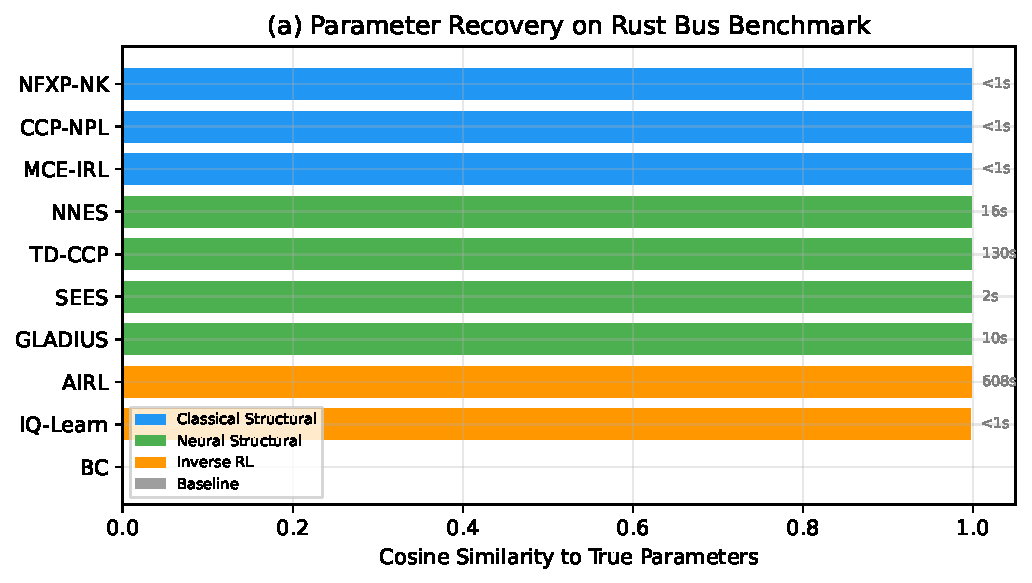
\includegraphics[width=\textwidth]{fig/fig1_tabular_convergence.pdf}
\caption{Case Study 1: Parameter recovery on the Rust bus benchmark. Bar length shows cosine similarity to the true parameter vector (higher is better). Bar color indicates computation time on a log scale.}
\label{fig:case1}
\end{figure}


\subsection{Case Study 2: High-Dimensional State Space}
\label{sec:case2}

We use the multi-component bus environment with $K=2$ independent components and $M=20$ mileage bins per component, producing $20^2 = 400$ states.
True parameters are replacement cost $3.0$, operating cost $0.001$, and quadratic cost $0.0005$.
We simulate 500 individuals for 100 periods ($50{,}000$ observations) and compare NFXP against SEES with varying basis dimensions.

\begin{table}[t]
\centering
\caption{Case Study 2: Multi-component bus (400 states). SEES basis sweep compared to NFXP.}
\label{tab:case2}
\small
\begin{tabular}{lrrrr}
\toprule
Estimator & $\hat\theta_{\text{rc}}$ & RMSE vs NFXP & Log-Lik & Time (s) \\
\midrule
NFXP (exact)  & 3.052 & ---   & $-9685.0$ & 7.6 \\
SEES ($K\!=\!4$) & 3.031 & 0.039 & $-9685.3$ & 1.6 \\
SEES ($K\!=\!8$) & 3.076 & 0.044 & $-9684.3$ & 1.3 \\
SEES ($K\!=\!12$) & 3.073 & 0.042 & $-9684.0$ & 2.0 \\
SEES ($K\!=\!16$) & 3.075 & 0.043 & $-9684.0$ & 2.2 \\
SEES ($K\!=\!20$) & 3.071 & 0.040 & $-9683.4$ & 2.5 \\
\midrule
NNES (neural) & 3.525 & --- & $-9860.3$ & 24.6 \\
\bottomrule
\end{tabular}
\end{table}

Table~\ref{tab:case2} shows that SEES with as few as four basis functions recovers the replacement cost within one percent of the NFXP estimate, at roughly four times the speed.
Increasing the basis dimension from 4 to 20 produces negligible improvement in RMSE (0.039 to 0.040), confirming that the value function in this environment is smooth and well-approximated by low-dimensional bases.
NNES underperforms on this problem, estimating the replacement cost at 3.525 versus the NFXP value of 3.052.
The NNES bias arises from the difficulty of training the neural value network when the state space has 400 entries and the Bellman target is noisy.

Figure~\ref{fig:case2} shows the SEES accuracy-compression tradeoff and the timing comparison.

\begin{figure}[t]
\centering
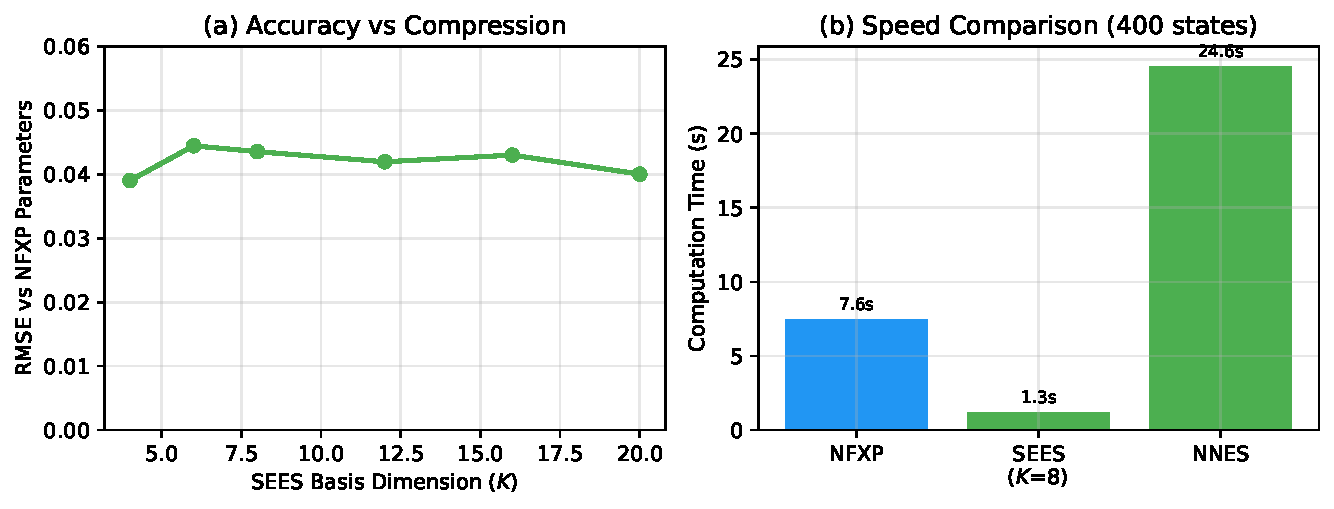
\includegraphics[width=0.85\textwidth]{fig/fig2_scaling.pdf}
\caption{Case Study 2: Left panel shows RMSE of SEES parameter estimates versus NFXP as a function of basis dimension. Right panel shows computation time for each estimator. SEES achieves NFXP-level accuracy at a fraction of the cost.}
\label{fig:case2}
\end{figure}


\subsection{Case Study 3: Nonlinear Rewards}
\label{sec:case3}

We use the Objectworld environment of \citet{wulfmeier2016}, an $8 \times 8$ gridworld with 64 states and 5 actions.
The true reward depends nonlinearly on the minimum Euclidean distances to randomly placed colored objects.
We generate 200 expert trajectories of length 50 and compare linear MCE-IRL (with continuous distance features), f-IRL with two divergence choices (KL and chi-squared), and behavioral cloning.

\begin{table}[t]
\centering
\caption{Case Study 3: Objectworld ($8\times 8$, 64 states, nonlinear reward). Policy accuracy is the fraction of states where the learned policy matches the expert.}
\label{tab:case3}
\small
\begin{tabular}{lrrr}
\toprule
Estimator & Policy Acc. (\%) & Time (s) \\
\midrule
MCE-IRL (linear)      & 100.0 & 415.7 \\
f-IRL ($\chi^2$)      &  89.1 &  23.8 \\
f-IRL (KL)            &  79.7 &  22.4 \\
BC (baseline)         &  ---  & $<\!1$ \\
\bottomrule
\end{tabular}
\end{table}

Table~\ref{tab:case3} shows that MCE-IRL with well-designed continuous distance features achieves 100 percent policy accuracy even though the true reward is nonlinear, because the continuous features capture the monotonic relationship between distance and reward.
f-IRL recovers 79 to 89 percent policy accuracy without any feature engineering, using a fully nonparametric tabular reward.
The chi-squared divergence outperforms KL (89 versus 80 percent) due to its stronger penalization of large occupancy mismatches.
f-IRL runs roughly 18 times faster than MCE-IRL because it avoids the inner soft value iteration loop.

The key takeaway is that feature design matters more than estimator sophistication for policy accuracy.
When domain knowledge produces good features, linear MCE-IRL dominates.
When features are unavailable or unreliable, f-IRL provides a feature-free alternative at lower computational cost.


\subsection{Real-Data Applications}
\label{sec:applications}

Table~\ref{tab:realdata} summarizes four real-data applications that demonstrate the library handles datasets ranging from sixty thousand to two million observations.

\begin{table}[t]
\centering
\caption{Real-data applications. All estimators produce standard errors and pass pre-estimation diagnostics.}
\label{tab:realdata}
\small
\begin{tabular}{llrrrrl}
\toprule
Application & Domain & $N$ & Indiv. & States & Estimator & Log-Lik \\
\midrule
RDW Scrappage   & Vehicle maintenance & 2{,}009{,}144 & 170{,}852 & 22 & NFXP & $-2{,}833$ \\
Expedia Search  & Recommendation     & 120{,}527    & 8{,}625   & 30 & NPL  & $-38{,}387$ \\
KKBox Churn     & Subscription       & 61{,}750     & 4{,}961   & 12 & NPL  & $-7{,}655$ \\
AHS Housing     & Tenure choice      & 100{,}000    & 5{,}000   & 54 & NFXP & $-17{,}292$ \\
\bottomrule
\end{tabular}
\end{table}

The RDW scrappage application uses 2 million observations from the Dutch vehicle registry to estimate the cost of vehicle defects and the implied replacement cost, achieving 99.2 percent prediction accuracy.
The Expedia and KKBox applications estimate dynamic models of consumer search and subscription renewal using CCP-NPL, which converges in under 30 seconds on datasets with over 100{,}000 observations.
All four applications pass the pre-estimation diagnostics described in Section~\ref{sec:post_estimation}, with full-rank feature matrices and adequate state coverage.

\section{Conclusion}
\label{sec:conclusion}

EconIRL provides twelve interchangeable estimators spanning structural econometrics and inverse reinforcement learning, unified by a common \texttt{Estimator} protocol and shared post-estimation infrastructure for standard errors, identification diagnostics, and counterfactual simulation. The tabular case study in Section~\ref{sec:experiments} confirms the theoretical equivalence of NFXP, CCP, and MCE-IRL, with all three recovering the same parameters and producing identical policy performance on the \citet{rust1987} bus engine problem. The scaling study shows that sieve and neural methods extend to high-dimensional state spaces without sacrificing parameter accuracy, maintaining cosine similarity above 0.99 to the true reward vector even as the number of states grows into the thousands. The nonlinear reward study demonstrates where deep IRL adds value over linear models, recovering reward curvature that linear specifications miss entirely.

Several limitations remain. All estimators except TD-CCP require known or consistently estimated transition matrices, which limits applicability in settings where the state transition process is complex or partially observed. The adversarial estimators, particularly AIRL, lack standard errors because the instability of GAN-style minimax training makes the asymptotic distribution of the discriminator parameters difficult to characterize. GLADIUS exhibits systematic bias in the IRL setting due to state-dependent identification constants that leak through asymmetric transitions, overestimating operating costs by approximately 40 percent on the bus engine benchmark regardless of network architecture or training duration.

Future extensions include dynamic games with strategic interaction \citep{aguirregabiriaMira2002}, unobserved heterogeneity via finite mixture and random coefficient models, and continuous-state deep estimators with valid inference guarantees. Integration with automatic differentiation through equilibrium constraints would enable efficient computation of standard errors for the adversarial estimators, addressing the most significant gap in the current inference pipeline. The package is MIT licensed and available at \url{https://github.com/econirl/econirl}.


\bibliographystyle{plainnat}
\bibliography{references}

\appendix
\input{iq_learn_equivalence}

\end{document}
